\documentclass[14pt,aspectratio=43]{beamer}

\usepackage{amssymb,amsmath,mathtext}
\usepackage{indentfirst,amsfonts}
\usepackage{makecell,multirow,longtable}

\usepackage[english,russian]{babel}
\usepackage[T2A]{fontenc}
\usepackage[utf8]{inputenc}


\graphicspath{{img/}}

%\usepackage{euscript}

\setbeamertemplate{navigation symbols}{}

%\usetheme{Warsaw}Boadilla,Pittsburgh,
%boxes,default,EastLansing
%Luebeck,Madrid,Szeged
\usetheme{EastLansing} 
%AnnArbor

%albatross,
%beaver, beetle, crane, dolphin, dove, fly, lily, orchid, rose, seagull, seahorse, sidebartab,
%structure, whale и wolverine
\usecolortheme{dove}%dove

\beamersetuncovermixins{\opaqueness<1>{30}}{\opaqueness<2->{25}}

%\setbeamerfont{frametitle}{series=\bfseries}
%\setbeamerfont{block title}{series=\bfseries}

%\makeatletter
%\defbeamertemplate*{footline}{my theme}{
%	\leavevmode%
%	\hbox{%
%	\begin{beamercolorbox}[wd=.205\paperwidth,ht=2.25ex,dp=1ex,center]{author in head/foot}%
%		\usebeamerfont{author in head/foot}%
%		\insertshortauthor~\beamer@ifempty{\insertshortinstitute}{}{(\insertshortinstitute)}
%	\end{beamercolorbox}%
%	\begin{beamercolorbox}[wd=.605\paperwidth,ht=2.25ex,dp=1ex,center]{title in head/foot}%
%		\usebeamerfont{title in head/foot}\inserttitle
%	\end{beamercolorbox}%
%	\begin{beamercolorbox}[wd=.19\paperwidth,ht=2.25ex,dp=1ex,center]{date in head/foot}%
%		\usebeamerfont{date in head/foot}\insertshortdate{}\hspace*{.3em}	\insertframenumber{}/\inserttotalframenumber\hspace*{1ex}
%	\end{beamercolorbox}}%
%}
%\makeatother



\begin{document}
\title{Сравнение тригонометрических параллаксов звезд TGAS и Hipparcos}
\subtitle[Диплом]{Дипломная работа}
%\subtitle[short subtitle]{long subtitle}
\author[А.С.\,Патшин]{Патшин Антон Сергеевич\\{\footnotesize\textcolor{gray}{научный руководитель: доцент А.С.\,Цветков}}}
\date{\today} 


%\title[short title]{long title}
%\subtitle[short subtitle]{long subtitle}
%\author[short name]{long name}
%\date[short date]{long date}

\institute[СПбГУ]{Санкт-Петербургский государственный университет}


\maketitle

\section{Введение}
\subsection{Общие сведения о Hips}
\label{sub:smthhip}
\begin{frame}\frametitle{Считалка} 

  \begin{itemize}
  \item Раз
  \item Два
  \item {\Large \textcolor{blue}{Рак за руку греку цап!}}
  \item Но! нету рук у греки в реки. Стоит нам ему помочь
  \end{itemize}
\begin{equation}
    Русский_{низ}^{вверх} = \frac{всё}{работает^2\dots} = E = m c^2
\end{equation}
\end{frame}


\subsection{Общие сведения о Gaia}
\label{sub:smthgaia}
\begin{frame}\frametitle{Название кадра}

 	\begin{columns}
 		\column{0.5\textwidth}
 			Содержимое левого столбца
 		\column{0.5\textwidth}
 			Содержимое правого столбца
 	\end{columns}
\end{frame}

\section{Данные}\label{sub:smthzd}
\subsection{Проекция Хаммер-Айтофа}\label{sub:hammer}
\begin{frame}[<alignment>]
\frametitle{Frame Title Goes Here}
Frame body text and/or \LaTeX code\\



Гомоморфный образ группы
изоморфен фактор-группе
по ядру гомоморфизма

\end{frame}	


\subsection{Визуализация распределения}\label{sub:smthrs}
\begin{frame}[<alignment>]
\frametitle{Frame Title Goes Here}
Frame body text and/or \LaTeX code\\

Гомоморфный образ группы
изоморфен фактор-группе
по ядру гомоморфизма

\end{frame}	


\subsection{Построение и предварительный анализ}\label{errvid}

\begin{frame}[c]
\frametitle{Frame Title Goes Here}
df
\begin{block}{Introduction to {\LaTeX}}
"Beamer is a {\LaTeX}class for creating presentations that
are held using a projector..."
\end{block}

\end{frame}	

\section{Случайные выбросы}\label{sub:smthrs}

\begin{frame}[<alignment>]
\frametitle{Случайные выбросы}


\begin{figure}[h!]
\center{\includegraphics[width=0.7\linewidth]{75maxlonlat}}
\label{img:75maxlonlat}
\end{figure}

\end{frame}	


\section{Систематические различия}\label{sistem}
\subsection{Healpix}\label{sub:smthhealpix}
\begin{frame}[<alignment>]
%\frametitle{Healpix}


\begin{figure}[h!]
\center{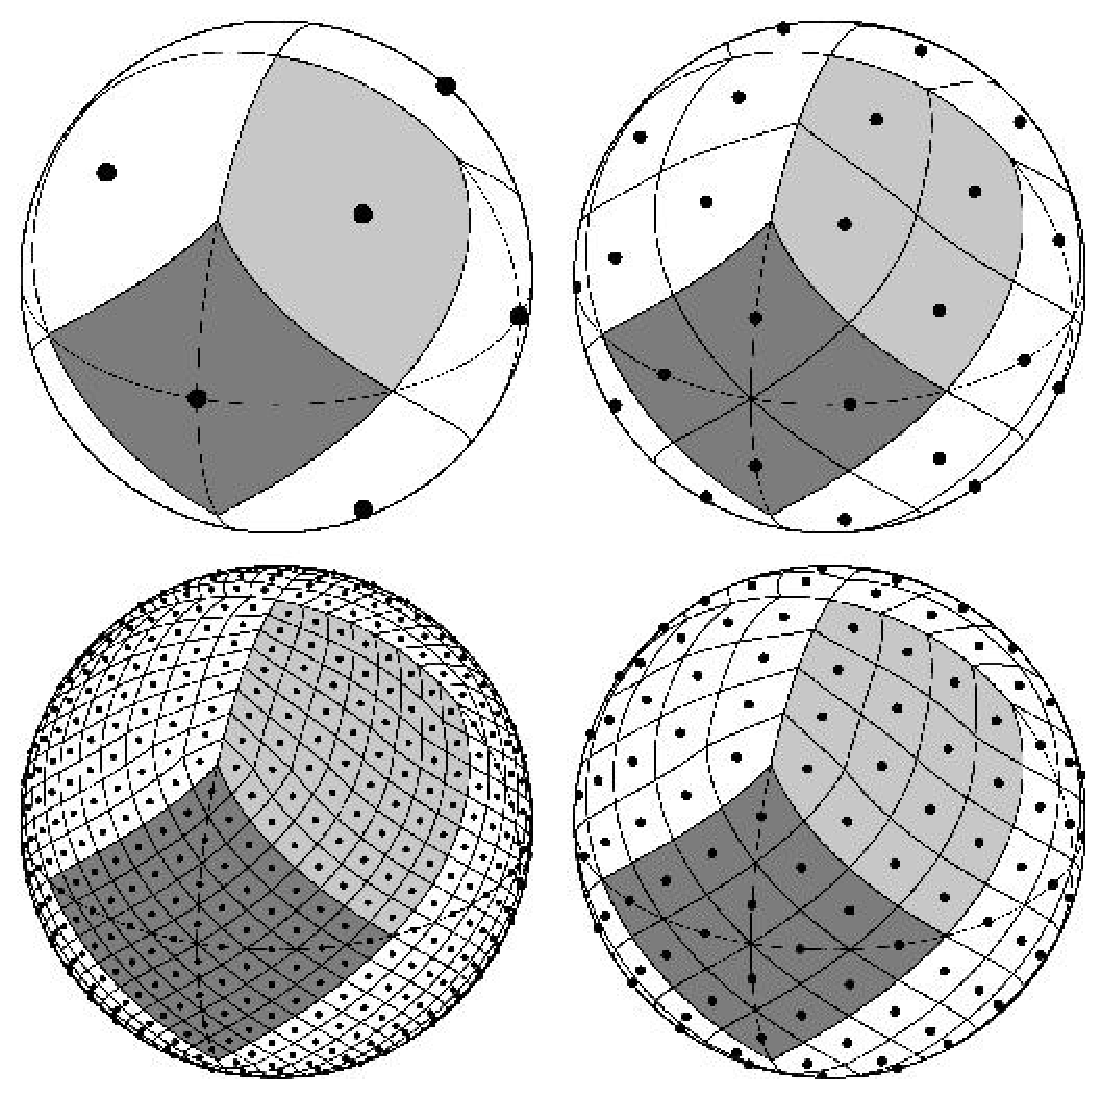
\includegraphics[width=0.6\linewidth]{healpix}}
\label{img:healpix}
\end{figure}

\end{frame}	

\subsection{Распределение разностей паралаксов}\label{sub:smthhealpix}
\begin{frame}[<alignment>]
\frametitle{Распределение разностей паралаксов}

\end{frame}	

\subsection{Сферические функции}\label{sistem}  
\begin{frame}[<alignment>]
\frametitle{Сферические функци}

\end{frame}	

\subsection{Сферические гармоники}\label{sistem}  
\begin{frame}[<alignment>]
\frametitle{Сферические гармоники}
d;e[

\end{frame}	

\section{Заключение}\label{conclusion}
\begin{frame}[<alignment>]
\frametitle{Заключение}
Звезды по HIP ближе на $6\%$.


\end{frame}	


\section{Список использованной литературы}\label{conclusionlit}
\begin{frame}[<alignment>]
\frametitle{Список использованной литератур}
wiki!!!
\end{frame}	

\end{document}